\section{The Games on Track GT-position system}
\label{GoTDescription}
The Games on Track GT-Position system, shortened GoT, is a position system which uses radio-waves and ultrasound to locate the object. The system is build up by three types of hardware components: the transmitter, the satellites and the master. The transmitter and the satellites send the information in all directions, with a 360 degree signal.\\
The GoT System does not work if the transmitter is not close enough from the satellites or if there is some interference by another signal or by an object between them and therefore can not communicate with the satellites.

\subsubsection{Transmitter}
The transmitter component is placed on the object, which needs to be located. The transmitter sends a ultrasound burst out, in 360 degree, that the satellites is intended to receive. The burst contains the id of the transmitter. The time at which each ultrasound bursts are sent from the transmitter to the satellites, is transmitted by radio waves to the master, to used later in the calculation. There is send a ultra sound burst each tenth of a second, giving a sampling frequency on 10 Hz.\\ 
The transmitter component runs on 2 AA-batteries and therefore does not need an external power-source.\\

\subsubsection{Satellites}
The satellites components are placed around the area where the object, with the transmitter on it, has to be located. The satellites should be place above the area, as under the ceiling. The satellites assignment is to search for the ultrasound waves, which the transmitter is emitting, and send a radio wave signal to the master as soon as they receive the burst with a time stamp.
To be able to calculate the exact position of the transmitter and then the object, a minimum of three satellites is necessary. However, more can be added to the system for more reliability or to cover a larger area. To work at a high efficiency, they should be placed 1 to 2 meters apart and not on a single line. But to cover a bigger area, they can be placed up to a distance of 5 meters between them, although this would affect the measurement and thereby make it less reliable. Each satellite have a maximum range of 8 meters and as seen on \figref{receiverSetup}. The three satellites should be placed in each others reach. The satellites needs between 14 to 20 volt DC. Thus, making the satellites able to be powered through a computer charger or by a panel solar for example is necessary.

\begin{figure}[H]
	\centering
	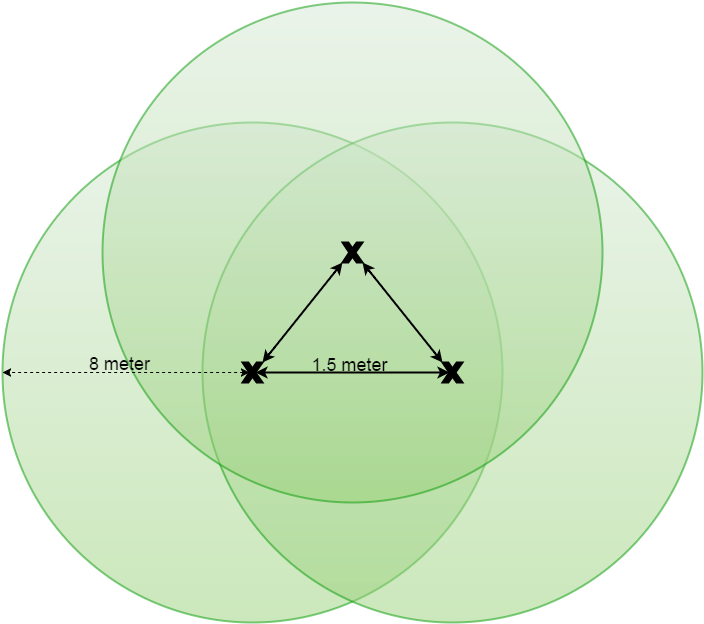
\includegraphics[scale=0.5]{figures/ReceiverSetup.png}
	\caption{Example on a standard setup for the satellites (increase size of text in figure)}
	\label{receiverSetup}
\end{figure}

\subsubsection{Master}
The master is a receiver which is connected to a computer. The masters assignment is to receive the data transmitted from the individual satellites and the transmitter, and relay it directly to the connected computer. The master is powered through a USB cable, between the master and the computer.\\

\subsubsection{Computer}
The program on the computer, which handles the information received from the master, uses the data to calculate the position of the transmitter. This is done with a method call Trilateration. Trilateration is a way of calculating a position, in a three-dimensional space, from three distances of known locations, with the help of spheres, circles and triangles. Therefore it is necessary for the system to have atleast three satellites, as mentioned earlier.  With additional satellites a check up can be performed to ensure the position of the transmitter is correct. Trilateration does not work if the three known points are on a single line, therefore the satellites should be placed in a triangle \todo{Fig insert}. The distances are calculated with the time when each satellites by a comparison to the time, the transmitter send the signal\\\\
\noindent
If the satellites have been moved, it is necessary to recalibrate the system. This is done with a calibration triangle. The calibration triangle is made of three points on a flat surface and have a distance of 40 to 200 centimeters between them. One of the points on the calibration triangle is made the origin (0,0,0) of the new coordinate system. Another point on the triangle will then be call (X,0,0), in which the line between the first point and the second point will become the X-axis. The last point will be call (X,Y,0) and will determine in which way the positive Y-axis will go. The surface which the calibration triangle is placed on, will be the XY-plan, where Z will go vertically, defining the (X,Y,Z) coordinates. The distance between the three points is measured and put into the program. Thereafter, the transmitter is placed in the three point, with (0,0,0) first and (X,Y,0) last. When the transmitter is placed in a point, the satellites measure the distance between them and the transmitter. From those information, the program can calculate the position of each satellites, with the help of trilateration. \\\\
\todo{insert the visio picture to explain the system}
\todo{Math example?}
